
\chapter{Results}

\section{Detailed Performance Analysis}

This section presents the results achieved by the navigation system under optimal conditions across various challenging datasets. The analysis focuses on the system's performance in terms of accuracy, efficiency, and generalizability, providing insights into its applicability in real-world UAV navigation scenarios.



\subsection{Key Performance Metrics}

The system's generalized performance across five diverse datasets—CITY1, CITY2, ROCKY, DESERT, and AMAZON— is summarized with two key metrics: Localization radial error in RMSE m and percentage, and localization inference time in seconds across all datasets. The results are presented in Figure \ref{fig:Key Metrics}. Importantly, the system meets the real-time requirement of 2 seconds and the accuracy requirement of 10\%. 

% the plot of key metrics with regard to system performance. 
\begin{figure}[H]
    \centering
    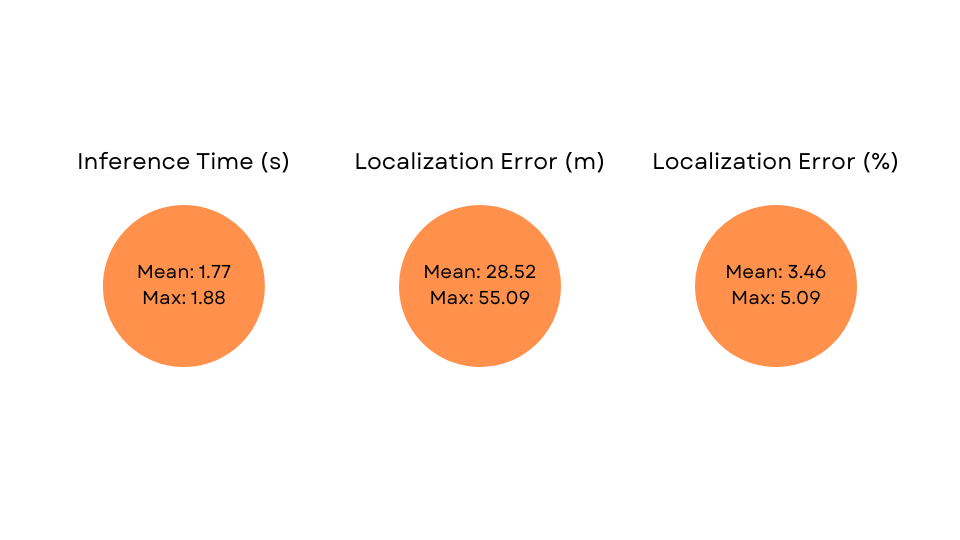
\includegraphics[width=0.8\textwidth]{./Chapter 5/RESULTPLOTS/Metrics_Raw.png}
    \caption{Key Accuracy And Runtime Performance Metrics}
    \label{fig:Key Metrics}
\end{figure}





\subsection{Flight Path Analysis}
Figures \ref{fig:Flight Path CITY1} and \ref{fig:Flight Path CITY2} show the actual vs estimated flight of the UAV across the worst and best performing dataset, CITY1 and CITY2 respectively. Even in the worst performing dataset, the system maintains a relatively accurate flight path, relative to its movement size, with the estimated path closely following the actual path. This indicates the system's ability to generalize and gives an idea of the scope of the error in the system.


    \begin{figure}[H]
        \centering
        \begin{minipage}{0.45\textwidth}
            \centering
            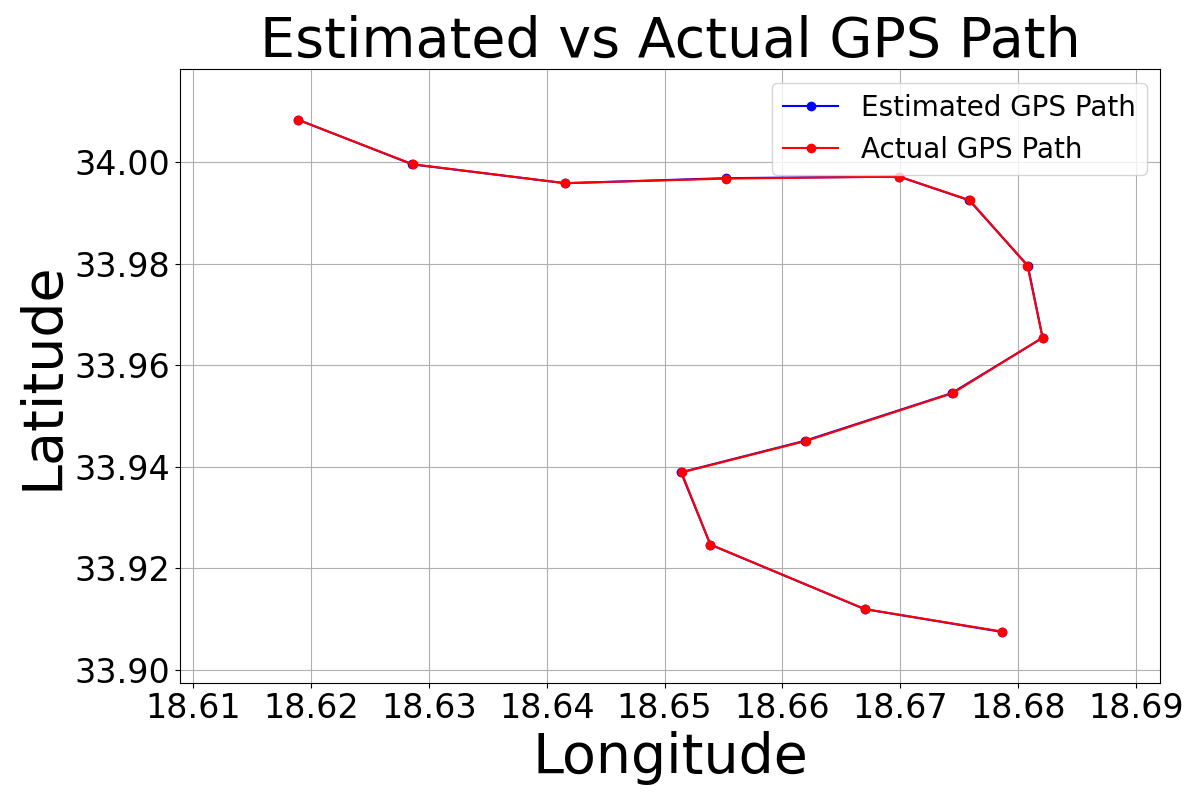
\includegraphics[width=0.7\textwidth]{./Chapter 5/GPSpaths/PathCity1.png}
            \caption{Flight Path of UAV in poorest performing Dataset}
            \label{fig:Flight Path CITY1}
        \end{minipage}\hfill
        \begin{minipage}{0.45\textwidth}
            \centering
            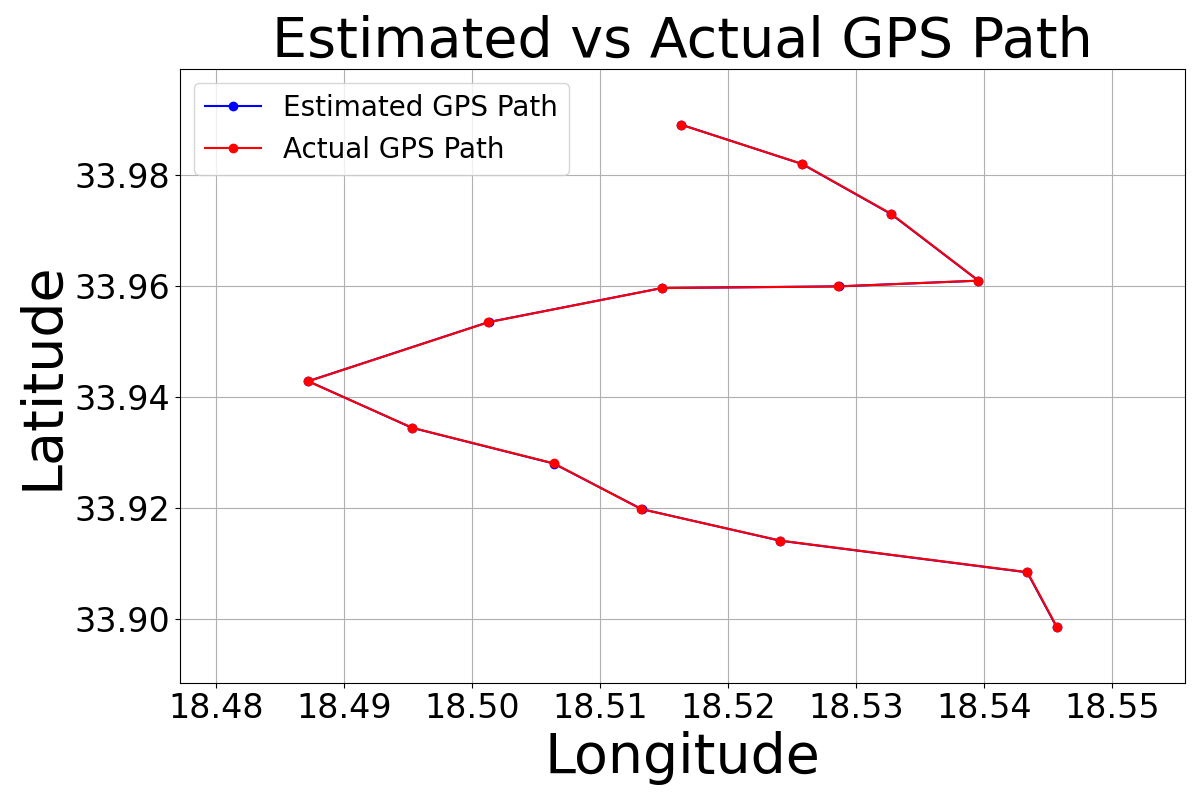
\includegraphics[width=0.7\textwidth]{./Chapter 5/GPSpaths/PathCity2.png}
            \caption{Flight Path of UAV in best performing Dataset}
            \label{fig:Flight Path CITY2}
        \end{minipage}
    \end{figure}


\subsection{Detailed Performance Metrics}
The detailed performance metrics include per dataset accuracy and time metrics. Namely, the radial RMSE error in GPS in meters and percentage, and the time taken for each stage of the pipeline, including the extraction and parameter inference time per while GPS is available, and the location inference time per image when GPS is lost. The results are summarized in Figures \ref{fig:Per Dataset Metrics} and \ref{fig:Per Dataset Metrics}. 

The results show that the system achieves consistent accuracy and runtime performance across each dataset. Further, its noted that both pipelines are able to maintain real-time performance, seen by the sum of the parameter inference and add times being below 2 seconds, as well as the location inference time being below 2 seconds. The accuracy of the system is also maintained, with the RMSE error being below 10\% for all datasets.


\begin{figure}[H]
    \centering
    \begin{minipage}{0.45\textwidth}
        \centering
        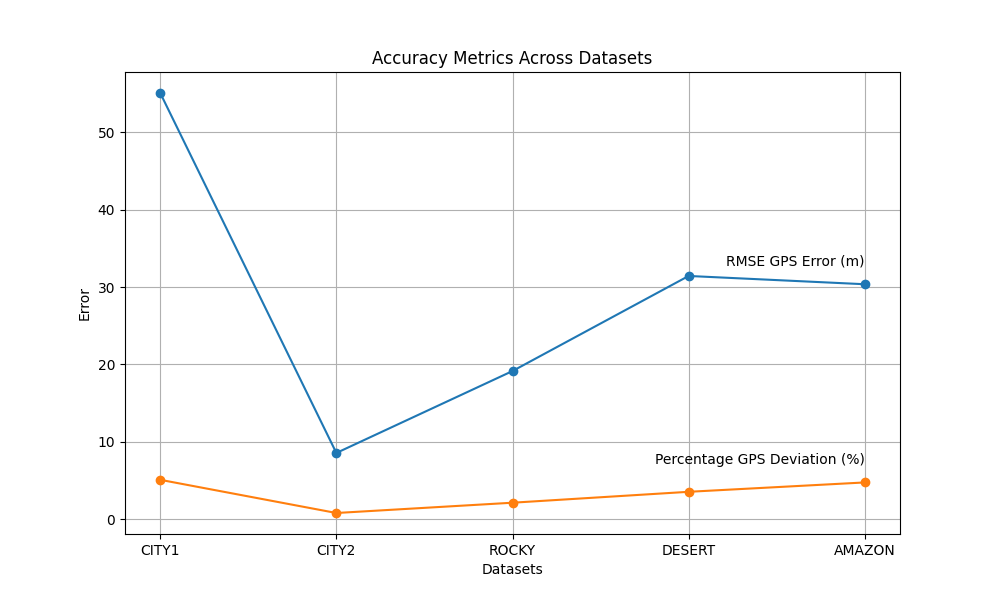
\includegraphics[width=\textwidth]{Chapter 5/RESULTPLOTS/key metrics/Accuracy Datasets.png}
        \caption{Accuracy Metrics for Each Dataset}
        \label{fig:Per Dataset Metrics}
    \end{minipage}\hfill
    \begin{minipage}{0.45\textwidth}
        \centering
        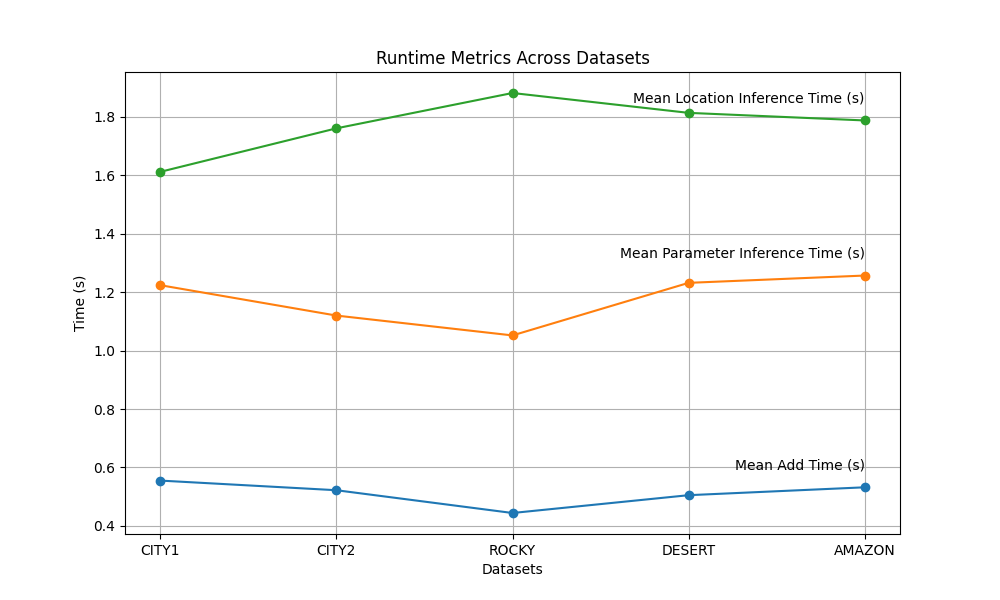
\includegraphics[width=\textwidth]{Chapter 5/RESULTPLOTS/key metrics/Runtime Datasets.png}
        \caption{Runtime Metrics for Each Stage of the Pipeline}
        \label{fig: Dataset Metrics}
    \end{minipage}
\end{figure}



\subsection{Dataset Performance Analysis}

This section utilizes the violin plot, in Figure \ref{fig:Violin Dataset Plot}, to visualize the statistical distribution of radial errors across each dataset. This plots details the mean, median, and variance of the radial errors, as well as the distribution of errors across the datasets. The results provide insights into the system's accuracy and robustness in diverse environments. 

The plot shows relatively consistent performance across datasets, with CITY2, being consistent with the global heading space, having the most accurate and reliable inter-dataset performance. The CITY1 and AMAZON datasets show comparitively high variation between their minimum and maximum errors, indicating a higher variance in direction.

\begin{figure}[H]
    \centering
    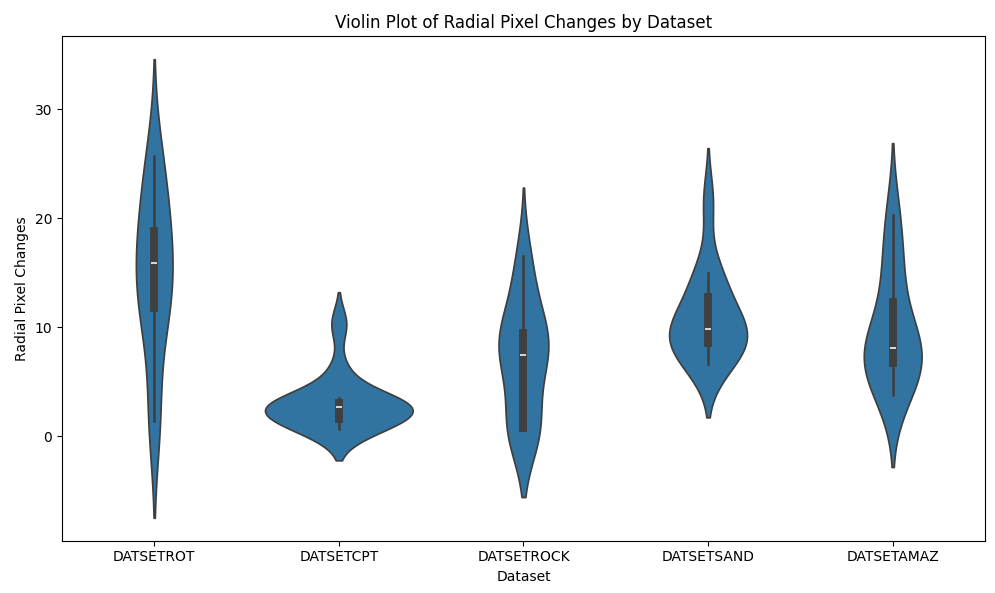
\includegraphics[width=0.7\textwidth]{Chapter 5/RESULTPLOTS/violindatasets.png}
    \caption{Plot of distribution of radial errors in each dataset}
    \label{fig:Violin Dataset Plot}
\end{figure}



\subsection{Error Distribution Map}

The heatmap in Figure \ref{fig:Heatmap_XY_Dev} visualizes the distribution of pixel deviations in the X and Y directions across the datasets. The results provide insights into the system's error patterns and highlight areas of potential improvement. The heatmap shows that the system has a relatively consistent error distribution across the datasets, with the majority of errors being within the 10-20 pixel range. However, some datasets, such as DESERT and AMAZON, exhibit larger errors of up to 30 pixels, indicating potential areas of significant error. 

\begin{figure}[H]
    \centering
    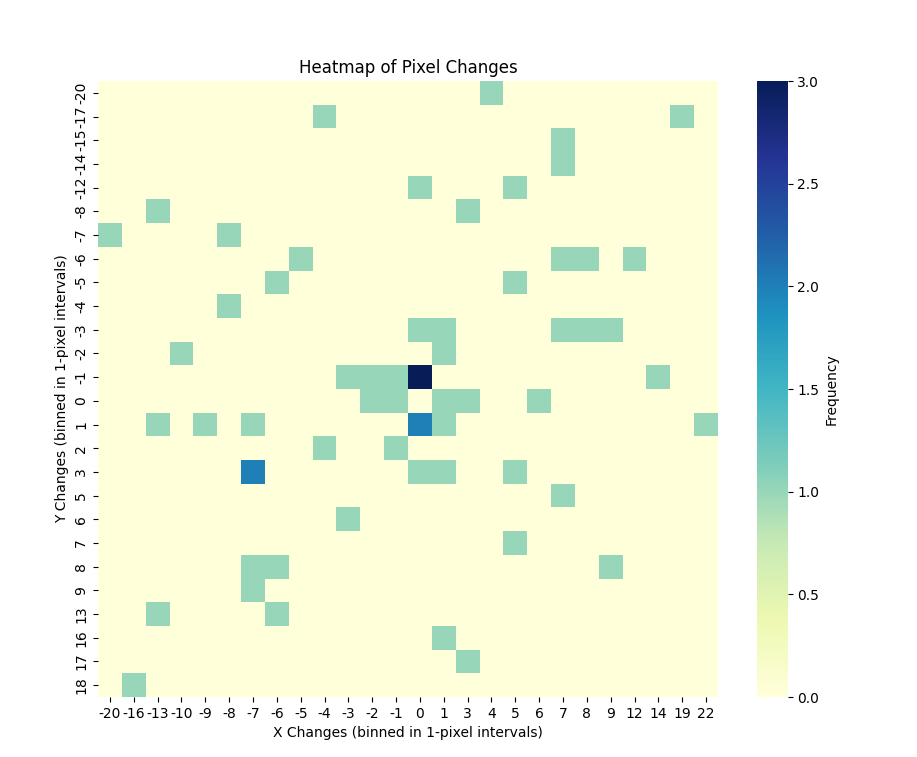
\includegraphics[width=0.55\textwidth]{Chapter 5/RESULTPLOTS/BIASPLOT_XY_HEAT.png}
    \caption{Heatmap of Pixel Deviations in X and Y Directions}
    \label{fig:Heatmap_XY_Dev}
\end{figure}


\subsection{An Account of Variance Between and Error in Datasets}
Given the large variation in error across datasets, as seen in both the violin plot in figure \ref{fig:Violin Dataset Plot} and the heatmap in figure \ref{fig:Heatmap_XY_Dev}, it is important to understand the sources of this variance. This section will detail the analysis conducted to identify the sources of this variance and the impact of these sources on the system's performance.

\subsubsection{Internal Uncertainty and Variance}
Correlations between error sizes and measures of uncertainty in the pipeline, specifically the standard deviation and mean-median difference in match vector magnitudes, were assessed. The variability in these vectors was used as a proxy for the uncertainty of the method. If the method was more uncertain when it was wrong, then the error likely originated from there. The match vectors, tested at various stages in the filtration process imply the accuracy of the transformational estimate. The results, in terms of correlation coefficients, as well as visual inspection, showed no relationship between uncertainty in the pipeline and error, indicating that there was not an increased likelihood of the variances in performance propagating from the anywhere including or before the transformational estimate.  

\subsubsection{Ground Truth Heading error and Variance}

Upon observing a moderate correlation between error magnitude and image sequence in the dataset, the accuracy of the estimated headings from Google Earth data was reconsidered. Ground truth headings, as explained in \ref{sec:scope}, were estimated. These heading estimates were generated early in the project, prior to the development of an optimized rotational estimation technique. Additionally, this technique involved sequential estimation, introducing cumulative errors. To evaluate the impact of these inaccuracies, a newer, optimized pipeline for heading estimation was employed, which would significantly reduce, but not eliminate, ground truth heading errors on the AMAZON dataset; The dataset was retested. The results demonstrated a significant reduction in mean radial error from 30.37 m to 17.91 m. This improvement underscores that inaccurate ground truth heading data was a significant contributor to the system's variance in performance across datasets.

\subsubsection{Impact of Heading Error on Accuracy}

Given these findings, and the factor improvements, it is estimated that the true absolute maximum error for an individual image in the given datasets, with the ground truth data available, is in the range of 7.5-15 pixels radially; this corresponds to around 3.4\%-6.8\% of the magnitude of the translation vector for that image, remaining within acceptable limits for the system's design objectives. Similar impacts are expected on the accuracy results of the other datasets, excluding the CITY2 dataset which has a fixed North heading for all images. The absence of true ground truth heading data constituted the primary factor in the variance in accuracy across datasets.

\subsubsection{Additional Sources of Error}

While heading estimation errors were identified as the main contributor to the overall inaccuracies, several other factors also contribute to the errors observed:

\textbf{Variations in Terrain and Environmental Conditions:} Differences in terrain, lighting conditions, and feature density affect keypoint detection and matching accuracy. The system, even with dynamic parameter adjustments, cannot perfectly predict the expected quantity or quality of features without specific dataset tuning. Consequently, it is due to inherently miss some high-quality features or incorrectly match less reliable ones. Incorporating a machine learning model to predict expected feature density could enhance the system's performance.

\textbf{Inaccuracies in Camera Parameter Estimations:} While the system dynamically infers camera parameters, any inaccuracies in these estimations accumulate, leading to scaled errors during subsequent localization steps that rely on these parameters.

\textbf{Image Noise and Resolution Limitations:} The Google Earth images used are at a fixed resolution of 1920x1080 pixels, which inherently contain some noise. This noise can adversely affect feature detection and matching accuracy.
\textbf{Algorithmic Constraints:} The selected image processing and matching algorithms have inherent limitations, particularly when handling extreme conditions or highly repetitive features. Additionally, being optimized for portability, they may not capture and represent every feature within an image perfectly.

Despite these factors, the achieved optimal radial error range, roughly 1-20 pixels across datasets, underscores the robustness and effectiveness of the image-based navigation system, affirming its suitability for practical UAV applications.

\section{Stress Testing}

This section involves the analysis of the system's robustness under various stressful conditions, including low-light environments and reduced mutual information. These tests were chosen practical and current relevance. The results aim to evaluate the system's performance under challenging scenarios and identify potential areas for improvement.

\subsection{Mutual Information Results}

In UAV navigation, accurate path maintenance is essential, especially when GPS signals are lost. Under these conditions, mutual information, or overlap—defined as the overlapping pixel information between current and reference images—plays a crucial role in guiding the UAV back on course. Specifically, when the UAV loses its path, there will be much less overlapping pixels than once the path is found.This study assesses whether reduced mutual information can still provide reliable navigational guidance and examines the trade-off between accuracy and computational efficiency.

The first objective was to identify the threshold of mutual information required to maintain an RMSE below 10\%, ensuring navigational accuracy without inducing additional drift. Secondly, it was to evaluate if reducing mutual information by cropping image sizes can significantly decrease runtime while preserving acceptable accuracy levels.

\subsubsection{Methodology}

The CITY2 dataset is utilized, focusing exclusively on translational changes to simplify the mutual pixel calculation to the difference between the image size and translation vector. Images are progressively cropped from the default resolution of 1920x972 pixels to reduce mutual information. The analysis uses the mutual information as that of the image pair with the lowest mutual information, since it is the systems bottleneck. This ensures visual brevity, noting that mutual information of that of the image pair with the highest mutual information remains within 30\% of the minimum across the dataset.

\subsubsection{Results}

Figure \ref{fig:Accuracy_Mutual} shows that navigational accuracy remains stable until mutual information decreases to approximately 250,000 pixels (15.67\% of a 1920x1080 image), below which accuracy sharply declines, indicating unreliable estimates. To maintain an RMSE below 10\%, mutual information must exceed 300,000 pixels (18.81\% of a 1920x1080 image). Reducing mutual information by cropping images significantly decreases runtime. While the identified mutual information thresholds are specific to this dataset and pipeline, the results demonstrate the feasibility of balancing mutual information and runtime for effective navigation. Lastly, it is noted that the system achieved largely varying levels of accuracy at the same mutual information level, indicating different amounts of information is stored in different axes. It is therefore recommended, if this method of decreasing runtime is considered, that the image is cropped towards an aspect ratio of one to maintain stability as the UAV rotates.


\begin{figure}[H]
    \centering
    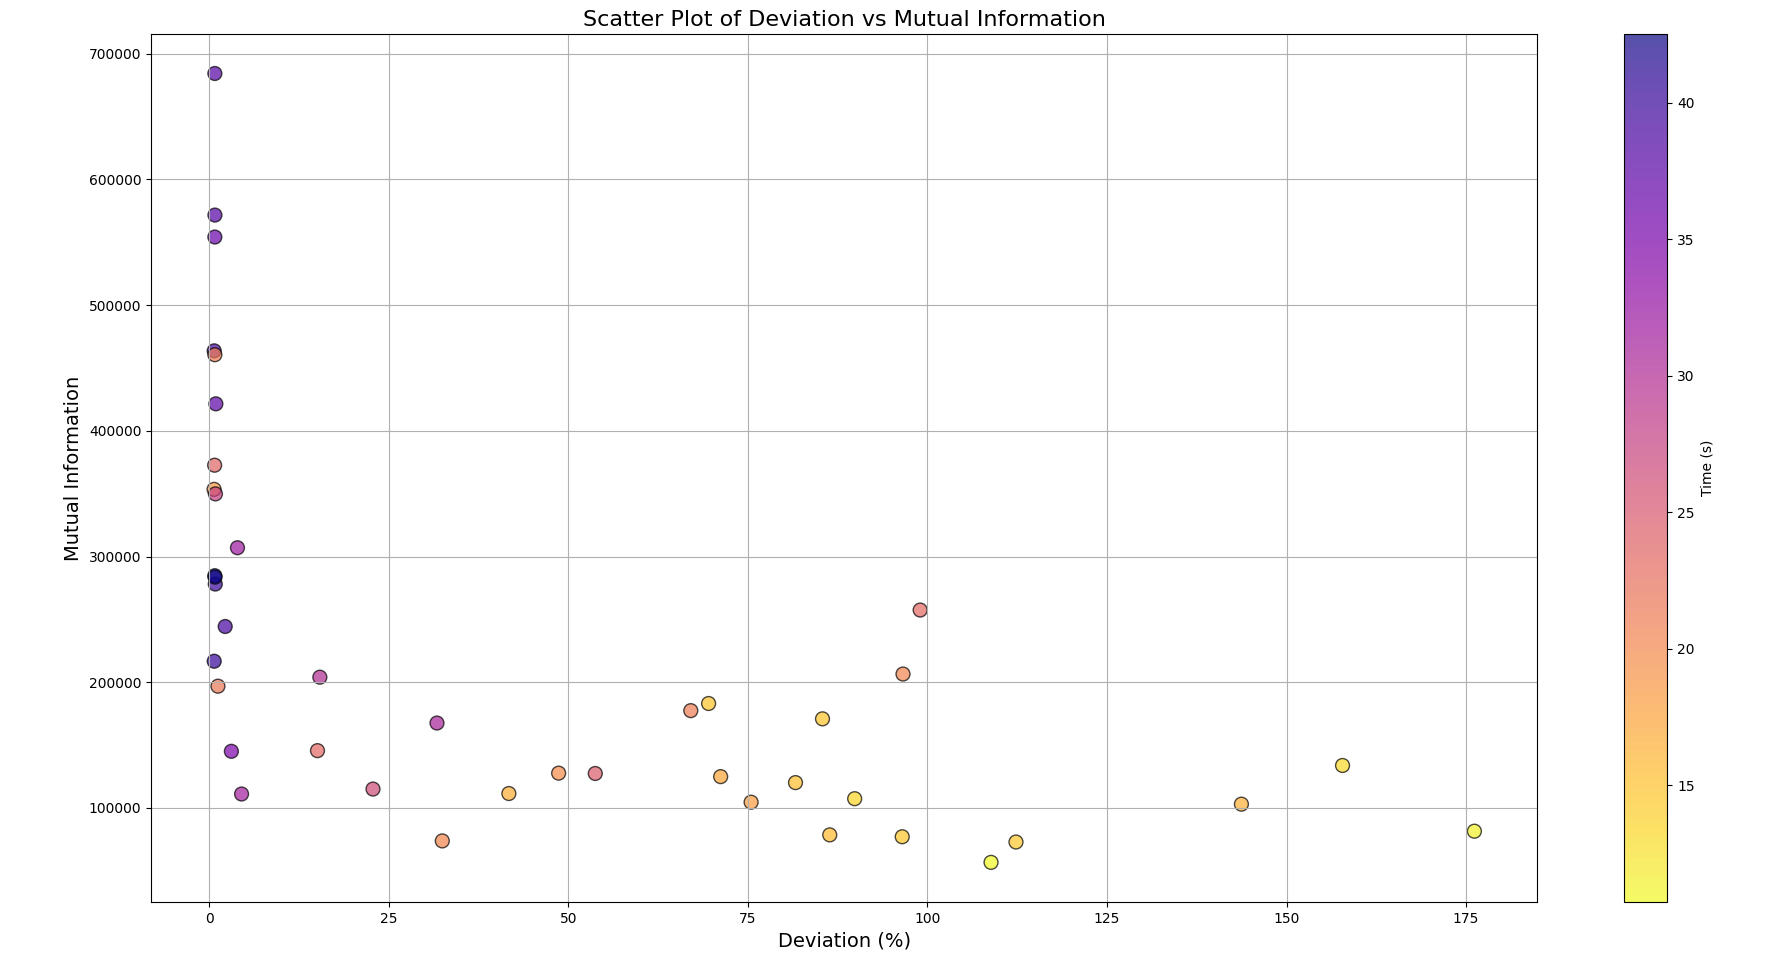
\includegraphics[width=0.7\textwidth]{Chapter 5/RESULTPLOTS/mutual/accmutual.png}
    \caption{Accuracy vs Mutual Information}
    \label{fig:Accuracy_Mutual}
\end{figure}



\subsubsection{Conclusions}

This study demonstrates that UAV navigational accuracy is maintained with mutual information levels up to approximately 20\% of the original image size. Above this threshold, additional mutual information yields diminishing returns in accuracy, indicating an inelastic performance region.
Runtime performance improves proportionally with reduced mutual information, presenting a trade-off between accuracy and computational efficiency. For instance, cropping the image resolution to 1100x635, subtending 300,000 mutual pixels achieves a 1.8-fold runtime reduction with only a 0.1\% increase in error.
These findings emphasize the importance of calibrating resolution levels to balance navigational accuracy and real-time performance. Further, when applying this method, cropping the image towards an aspect ratio of one is recommended to maintain stability as the UAV rotates. Future work should explore adaptive methods that start with reduced mutual information and increase it only when necessary, such as when the UAV is turning around to find its path. 


\subsection{Low-Light Testing}

UAV navigation performance can be significantly impacted by low-light conditions, where keypoint detection and matching accuracy decline due to reduced visibility and increased noise. This study evaluates the robustness of the navigation method under simulated evening and nighttime conditions across five datasets: CITY1, CITY2, ROCKY, DESERT, and AMAZON. Conditions are simulated through adaptions in image brightness, contrast, tint, and noise levels to mimic real-world low-light environments. Evening conditions involve moderate applications of these adjustments, while nighttime conditions feature severe reductions in visibility and increased noise levels. 

The objectives of this study are twofold: firstly, to assess the robustness of the UAV navigation system under low-light conditions by evaluating how evening and nighttime lighting affect the accuracy of navigational estimates; and secondly, to compare the system's performance across diverse environments with varying feature densities under these low-light scenarios.

Representative examples from the CITY1 dataset illustrate these conditions:

\begin{figure}[H]
    \centering
    \begin{minipage}{0.32\textwidth} % Adjust width as necessary
        \centering
        \includegraphics[width=\textwidth]{Chapter 5/RESULTPLOTS/lighting/dayCPT.png}
        \caption{Daytime Image of Cape Town}
        \label{fig:Day_CPT}
    \end{minipage}\hfill
    \begin{minipage}{0.32\textwidth} % Adjust width as necessary
        \centering
        \includegraphics[width=\textwidth]{Chapter 5/RESULTPLOTS/lighting/eveningCPT.png}
        \caption{Evening Image of Cape Town}
        \label{fig:Evening_CPT}
    \end{minipage}\hfill
    \begin{minipage}{0.32\textwidth} % Adjust width as necessary
        \centering
        \includegraphics[width=\textwidth]{Chapter 5/RESULTPLOTS/lighting/nightCPT.png}
        \caption{Night Image of Cape Town}
        \label{fig:Night_CPT}
    \end{minipage}
    
    \caption{Lighting Conditions in Cape Town}
    \label{fig:Lighting_CPT}
\end{figure}


\subsubsection{Results}

Figure \ref{fig:night_evening_rmse} summarizes the accuracy of the navigation method under evening and nighttime conditions for each dataset. Nighttime performance shows that the CITY and ROCKY datasets maintain relatively low RMSE values, indicating resilience to severe low-light environments, while the DESERT and AMAZON datasets exhibit substantial increases in RMSE due to sparse and repetitive features hindering effective keypoint matching. Evening conditions result in minimal degradation of navigational accuracy for most datasets, with the DESERT dataset experiencing a moderate error increase from its initial RMSE of 31.44 m to 156.34 m, corresponding to a 17.51\% RMSE error, which remains usable. 

The performance disparity between datasets underscores the importance of feature density in low-light navigation, with environments rich in distinct landmarks (e.g., CITY and ROCKY) demonstrating greater robustness compared to feature-poor environments (e.g., DESERT and AMAZON).

Overall, the navigation method demonstrates profound resilience in well-featured environments under low-light conditions. However, challenges still remain in feature-sparse environments during nighttime. The usage of additional sensors, such as infrared cameras, could enhance navigational accuracy in these challenging scenarios. 




    \begin{figure}[H]
        \centering
        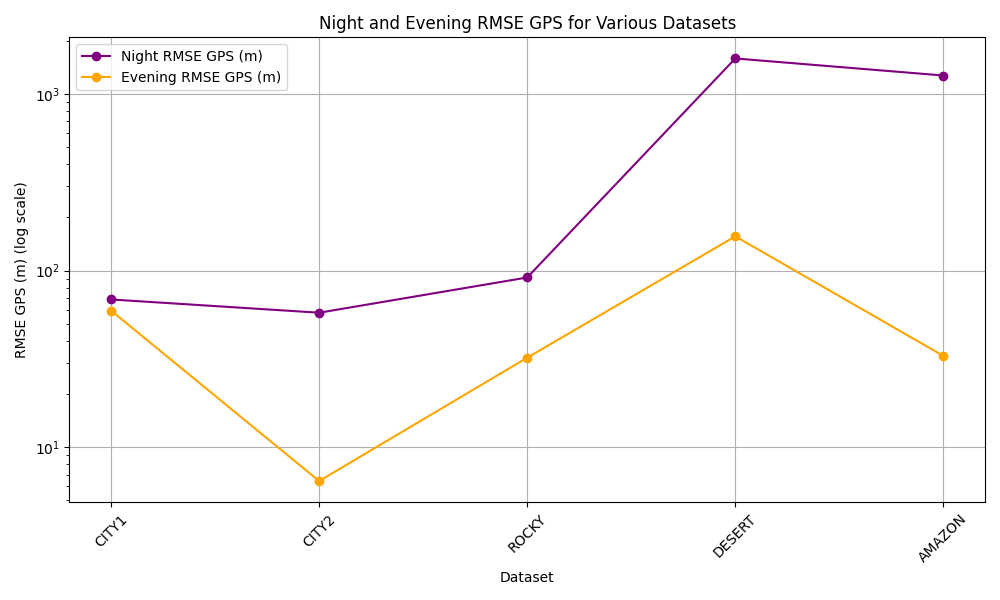
\includegraphics[width=0.7\textwidth]{./Chapter 5/RESULTPLOTS/night_evening_rmse.png}
        \caption{Night and Evening RMSE GPS for Various Datasets}
        \label{fig:night_evening_rmse}
    \end{figure}

    

\section{Results Conclusion}

The results presented in this chapter confirm that the system meets the accuracy and time requirements established in the objectives. The system demonstrated reliable performance across various datasets, including sparse-feature environments, showcasing its ability to generalize effectively. Despite practical limitations such as resolution constraints, performance limitations, and fluctuating terrain feature densities, the system maintained robust accuracy.

The analysis further indicates that accuracy would be significantly improved with access to accurate ground truth headings and known camera parameters, reducing potential sources of error. Furthermore, the system showed resilience under challenging conditions, including low-light scenarios and images with reduced mutual information. Even with limited pixel overlap, the system continued to deliver reliable navigation data.

Overall, the system has proven to be a versatile and effective solution for UAV navigation, capable of sustaining performance under a wide range of operational challenges and environmental conditions.

